\subsection{Problema a resolver}
El siguiente ejercicio consiste en escribir un algoritmo capaz de devolver, dado un conjunto de intervalos, el subconjunto máximo de los que no se solapan. Luego, el algoritmo debe poder tomar las fechas ofrecidas por los profesores del programa de Profesores Visitantes de la FCEyN para sus cursos e indicar qué cursos deberían elegirse para maximizar la cantidad de cursos en el ciclo. Cada intervalo corresponde a la fecha en que un profesor  dictará su curso. El primer elemento del intervalo corresponde a la fecha de inicio y el segundo a la fecha de fin. Para la simplificación del manejo de los datos, éstos se representan con números enteros positivos.\newline
\newline
\textbf {Formatos de entrada y salida:}\newline
\newline
La entrada contiene varias instancias del problema. Cada instancia consta de una línea con el siguiente formato:

$$n\ i_{1}\ f_{1}\ i_{2}\ f_{2}\ ...\ i_{n}\ f_{n}$$


donde \textbf{$n$} es la cantidad de cursos ofrecidos por los profesores (numerados de 1 a n) y los valores \textbf{$[i_{1},f_{1}],\ ...,\ [i_{n},f_{n}]$} representan los días de inicio y fin de cada uno de los n cursos. Todos los datos son enteros positivos. La entrada concluye con una línea comenzada por \# que no debe ser procesada.\newline

La salida debe contener una línea por cada instancia de entrada, donde se listan los números de los cursos elegidos para el ciclo de cursos.\newline
\newline
En lo que sigue, presentaremos dos ejemplos sobre cómo debería comportarse nuestro algoritmo:\newline

{\large{\textbf{Ejemplos:}}}\newline

\begin{figure}[H] %[h] Aqui [b] para button [t] para top
\begin{center}
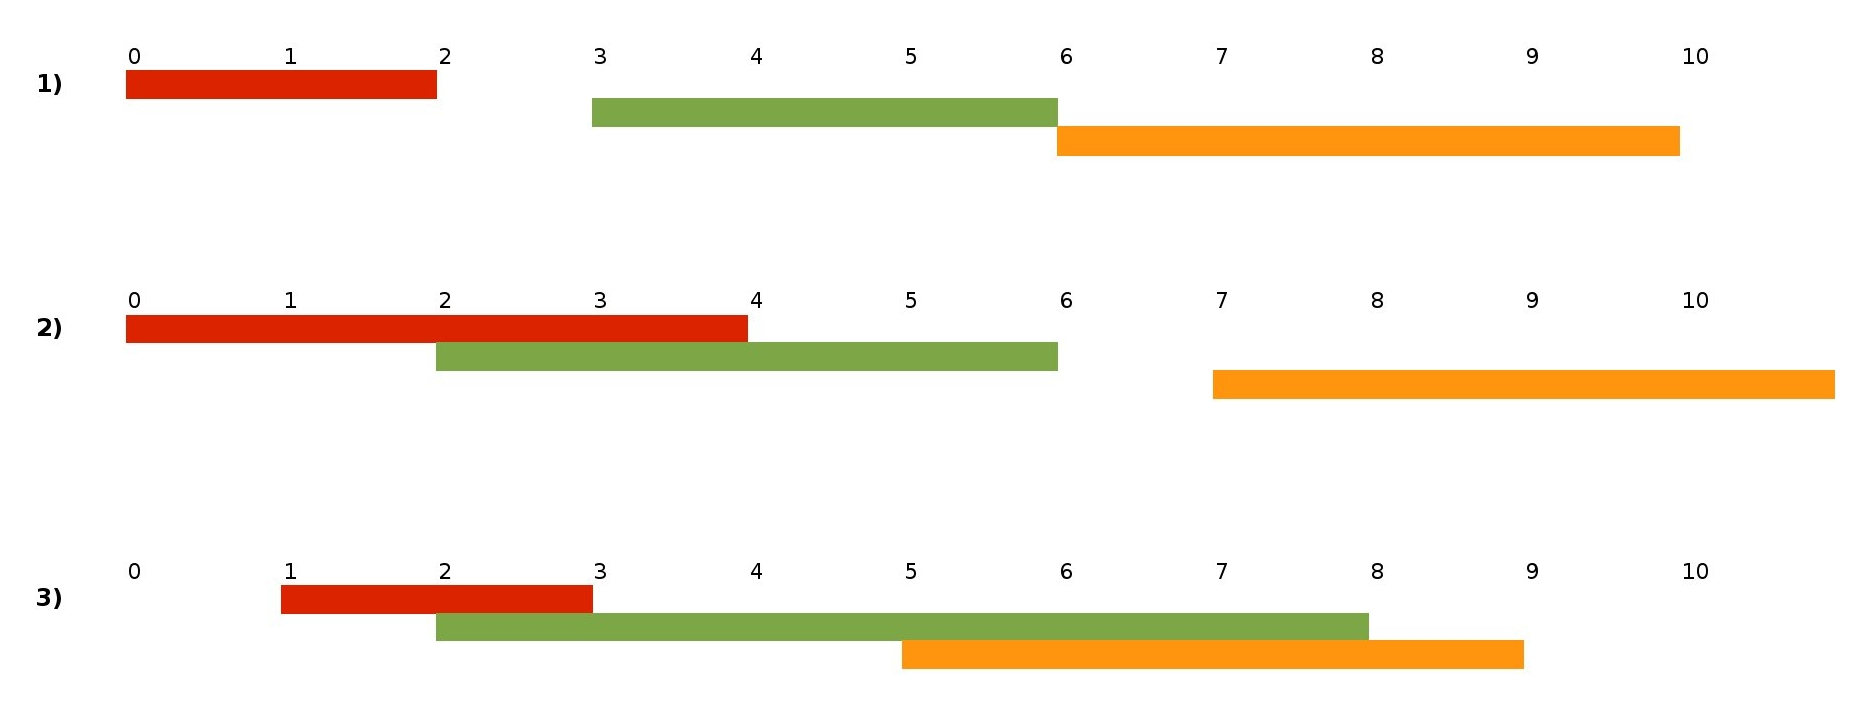
\includegraphics[width=450pt]{../imgs/ejemplosej2.jpg}
\end{center}
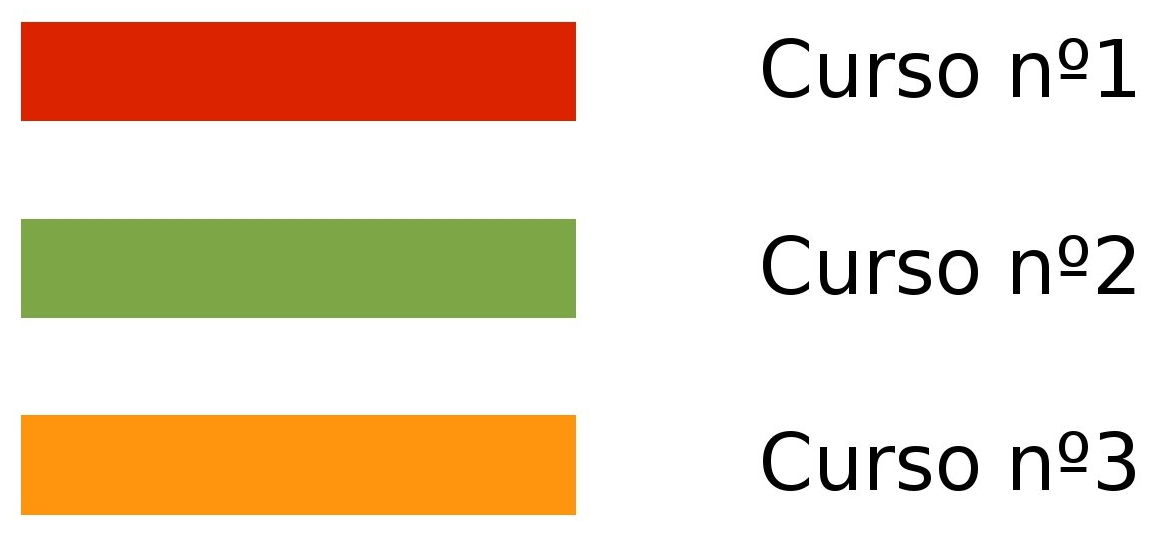
\includegraphics[width=80pt]{../imgs/leyendaejemploej2.jpg}
\end{figure}
En el ejemplo \textbf{1)}, decidimos mostrar un caso en el que no se solapara ningún curso. En esta ocasión, puede observarse que, dado que hay una solución óptima, ésta es única.\newline

\textbf{Formato de entrada:}
$$3\ \ 0\ \ 1\ \ 3\ \ 5\ \ 6\ \ 9$$

\textbf{Formato de salida:}
$$1\ \ 2\ \ 3$$

En el ejemplo \textbf{2)}, resolvimos develar un caso en el que hubiera un único solapamiento con el fin de mostrar una situación cuyas soluciones óptimas fueran más de una. En esta oportunidad, hay dos salidas posibles que son solución del problema. Debido que nuestro algoritmo almacena, en primer lugar, los intervalos cuya fecha de fin es la más alta, dicho intervalo es el prioritario frente a cualquiera que se le solape.\newline

\textbf{Formato de entrada:}
$$3\ \ 0\ \ 3\ \ 2\ \ 5\ \ 7\ \ 10$$

\textbf{Formato de salida:}
$$2\ \ 3$$

En el ejemplo \textbf{3)}, preferimos mostrar un caso en el que se solaparan todos los cursos. En esta situación, cualquier curso del ciclo es solución del problema pues es la máxima cantidad de intervalos que no se solapan.\newline

\textbf{Formato de entrada:}
$$3\ \ 1\ \ 2\ \ 2\ \ 7\ \ 5\ \ 8$$

\textbf{Formato de salida:}
$$3$$

\subsection{Resolución coloquial}

O1: Los dias de inicio son menores a los dias de finalizacion de cada curso\\

Sea $v$ un intervalo, este intervalo está representado por dos valores: $v_{i}$ es el inicio del intervalo y $v_{f}$ es el fin del intervalo. Sea C un conjunto de intervalos.\\

El modelo de nuestro problema mapea a los cursos como intervalos, donde el dia de incio es el valor $v_{i}$ y el dia de finalizacion del curso es $v_{f}$, la solucion se obtiene encontrando un conjunto maximo de elementos cuyos intervalos no se solapen, esto significa: 

\par{$$\forall v1, v2 \in C\ |\ (v1_{f} < v2_{i}) \vee (v2_{f} < v1_{i})$$} 

esta es condición suficiente ya que por O1 el valor de incio de un curso es menor al valor de fin del mismo curso para todos los cursos.

\subsection{Demostración de correctitud}

Veamos que, efectivamente, nuestro algoritmo encuentra una solución óptima $S$. Supongamos, por el absurdo, que existe una solución $S'$ cuya cantidad de intervalos es mayor que la de $S$.\\ Si hubiera intervalos en $S' - S$ que no se solaparan con ninguno de $S$, entonces éstos deberían estar en $S$ dado que es la solución que maximiza la cantidad de cursos que no se solapan. De este modo, llegamos a un absurdo proveniente de suponer que existe una mejor solución al problema.

\par{En el caso en el que los intervalos $S' - S$ se solaparan con intervalos de $S$, deberían existir al menos $n-1$ intervalos (que llamamos $V$) en $S$ que puedan ser reemplazados por $n$ o más intervalos (que llamamos $W$) en $S'$. Sabemos que $\#V < \#W$ ya que, caso contrario, no podríamos decir que existe una mejor solución. Luego, debe existir un intervalo $w \in W$ tal que para algún intervalo $v \in V$ se cumpla que $f_{w} > i_{v} \land f_{v} > i_{w}$. Esto quiere decir que $f_{w} < f_{v}$, pero si esto fuera así, el algoritmo hubiera seleccionado primero el intervalo $w$ ya que siempre toma los intervalos que terminan antes de los que ya seleccionó. De esta manera, llegamos a un absurdo que provino de suponer que existía una mejor solución al problema.}


\subsection{Complejidad del algoritmo}

Sea $n$ la cantidad de cursos. La complejidad de nuestro algoritmo es $\mathcal{O}(n\ log\ n)$, antes de ver el porque de esto tengamos en cuenta algunos aspectos:
\begin{enumerate}
\item La complejidad del algoritmo \textbf{Sort} es $\mathcal{O}(n\ log\ n)$\footnote{http://en.cppreference.com/w/cpp/algorithm/sort}.
\item La complejidad del \textbf{constructor} que utilizamos sobre la estructura \textbf{vector} es $\mathcal{O}(1)$\footnote{http://en.cppreference.com/w/cpp/container/vector/vector}.
\item La complejidad del \textbf{reserve} que utilizamos sobre la estructura \textbf{vector} es $\mathcal{O}(n)$\footnote{http://en.cppreference.com/w/cpp/container/vector/reserve}.
\item La complejidad del algoritmo \textbf{push$\_$back} sobre la estructura \textbf{vector} es O(1) amortizado pero cuando se ultiliza previamente la funcion $reserve(n)$ agregar los primeros n elementos es O(1)\footnote{http://en.cppreference.com/w/cpp/container/vector/push$\_$back}. 
\item La complejidad del algoritmo \textbf{size} sobre la estructura \textbf{vector} es O(1)\footnote{http://en.cppreference.com/w/cpp/container/vector/size}.
\item La complejidad de la funcion \textbf{filtrarSolapamientos} es $\mathcal{O}(n)$ ya que va recorriendo los cursos, comparando y agregando elementos segun corresponda (comparar es constante al igual que agregar y recorrer lineal), en otras palabras, se encuentra un \textbf{if} (complejidad constante) y un \textbf{push$\_$back} (complejidad constante) dentro de un \textbf{for} (complejidad lineal). 
\end{enumerate}
Teniendo en cuenta lo anterior el siguiente grafico muestra el codigo y al costado la complejidad de cada operacion.

\begin{figure}[H] %[h] Aqui [b] para button [t] para top
\begin{center}
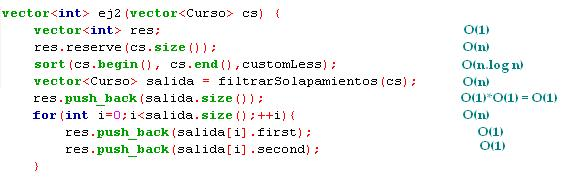
\includegraphics[]{../imgs/comple2.jpg}
\end{center}
\end{figure}

Finalmente, la complejidad es: $\mathcal{O}(1)+\mathcal{O}(n)+\mathcal{O}(n\ log\ n)+\mathcal{O}(n)+\mathcal{O}(1)+\mathcal{O}(n)*\mathcal{O}(1)*\mathcal{O}(1)$ = \textbf{\mathcal{O}(n\ log\ n)}

\subsection{Código fuente}



\subsection{Instancias posibles}



\subsection{Testing}
